\documentclass[conference]{IEEEtran}
\IEEEoverridecommandlockouts
% The preceding line is only needed to identify funding in the first footnote. If that is unneeded, please comment it out.
\usepackage{cite}
\usepackage{amsmath,amssymb,amsfonts}
\usepackage{algorithmic}
\usepackage{graphicx}
\usepackage{textcomp} 
\usepackage{hyperref}
\usepackage{xcolor}
\usepackage[style=ieee]{biblatex}
\addbibresource{references.bib}
\def\BibTeX{{\rm B\kern-.05em{\sc i\kern-.025em b}\kern-.08em
    T\kern-.1667em\lower.7ex\hbox{E}\kern-.125emX}}
\begin{document}

\title{implem \\}

\maketitle

\begin{abstract}
This paper will dive in four different implementation of the insertion sort algorithm. They four implementations are FSMD (Finite State Machine with Data path), ASIP (Application-Specific Instruction-set Processor), C (software-based implementation) and Custom IP (hardware-based implementation). They will be explained and afterwards compared under the following aspects:
% // TODO: add the aspects
\end{abstract}

\section{Introduction}

\section{InsertionSort}
We decided to implement the InsertionSort Algorithm for the project asignment, because it is a well-known, not too complex sorting algorithm. The idea of InsertionSort is similar to "sorting playing cards in your hands. You split the cards into two groups: the sorted cards and the unsorted cards. Then, you pick a card from the unsorted group and put it in the right place in the sorted group." \cite{g4g}\\
It is maily used for small or nearly sorted lists because the time complexity of insertionsort is a $O(n)$ in the best-case (= numbers already sorted algotithm) but $O(n^2)$ for the average and worst case. \\
InsertionSort is a in-place sorting algotithm which means that its space complexity is at $O(1)$. 


\section{Implemtations}
In this next session we will start introducing our four different implementations. We started the project by firstly get clarity of the logical design and describe it in a finite state machine with data path (FSMD) diagramm as well as an algorithm state machine with datapath (ASMD) diagramm. Then we started our implementations.
\subsection{FSMD}
First part to implement was the finite state machine with data path. We used the napoleon cypher FSMD as a base project and adapted the fsm and the top file by implementing the behaviour that was described in the previously defined FSMD diagram \autoref{fig:fsmd}. We tested our functionality by using the waveform configuration and added the uart receiving and transmitting file so we could use our serial connection to putty.exe as in- and output. 
\begin{figure}
    \centering
    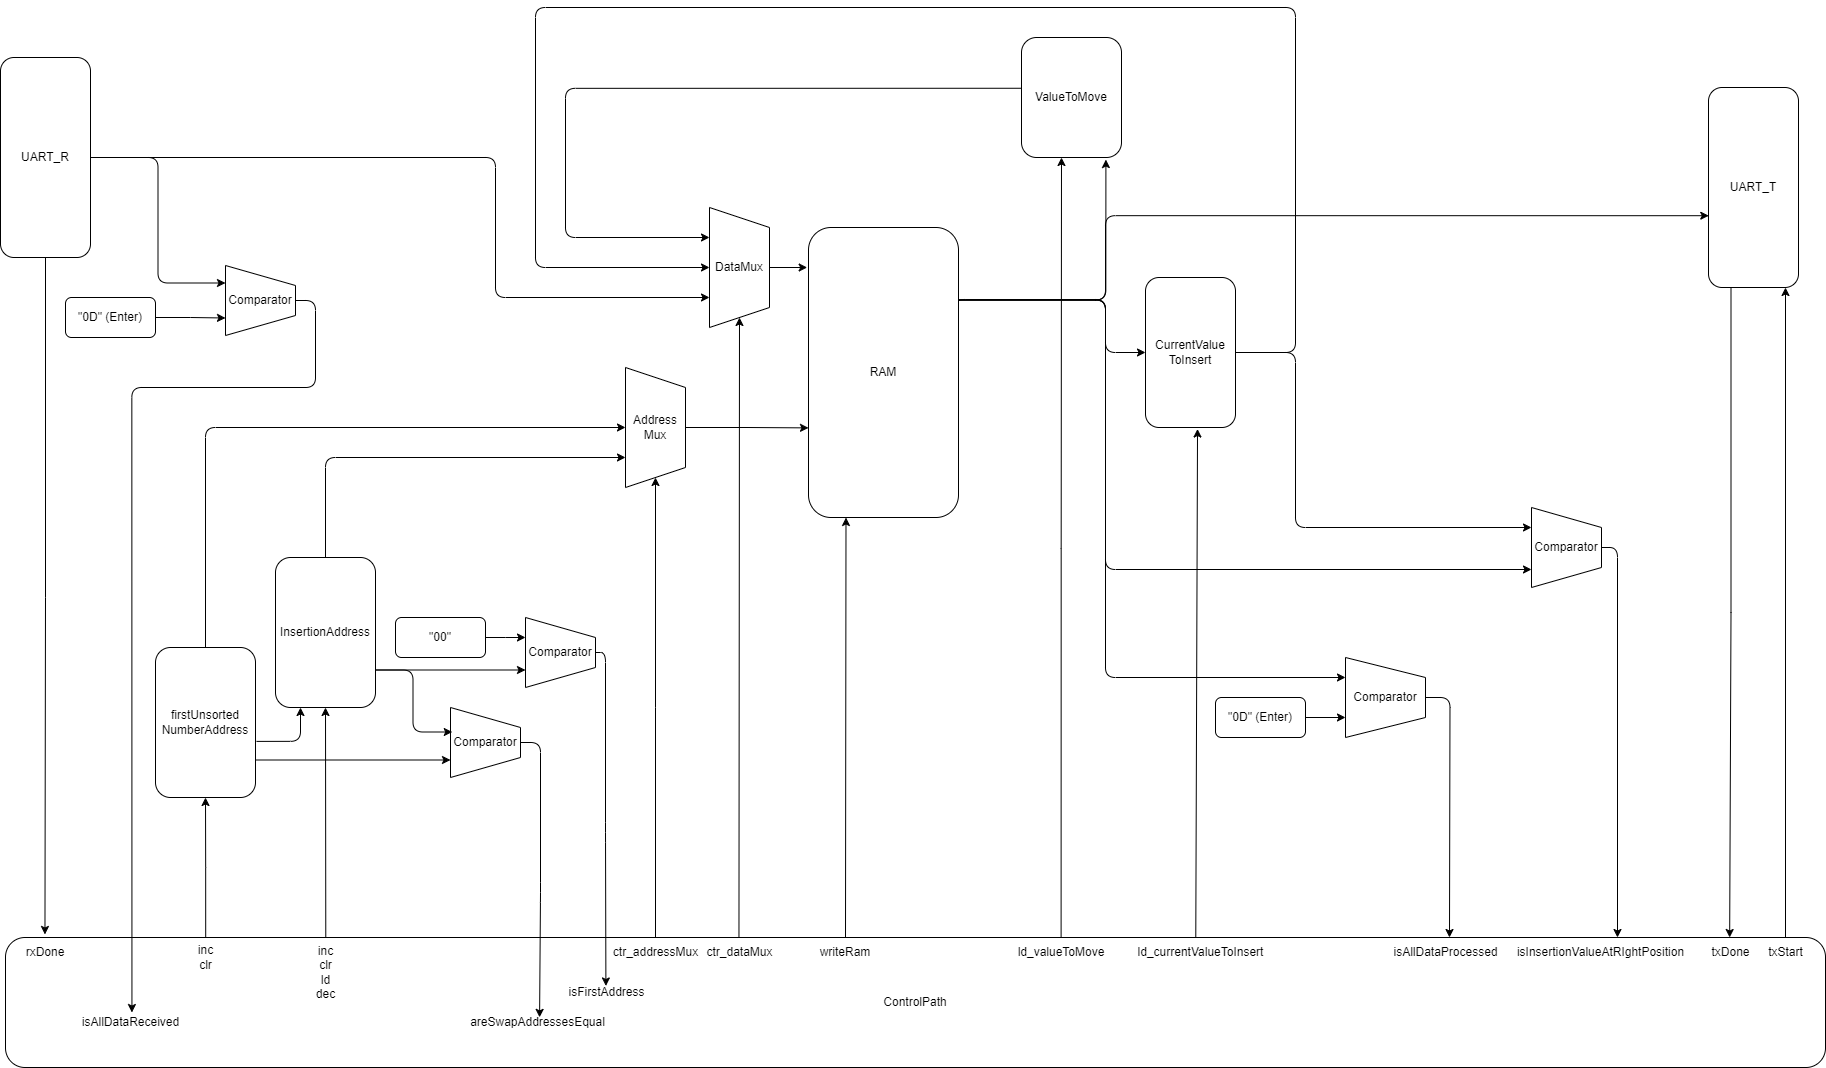
\includegraphics[width=1\linewidth]{Images/FSMDInsertionSort.png}
    \caption{FSMD diagram for the insertion sort}
    \label{fig:fsmd}
\end{figure}

\subsection{ASIP}
Second implementation was the application-specific instruction set processor, which we implemented using the states described in the ASMD chart. This allowed us to stay consistent with our design choices as well as keep a structred overview of the ASIP implementation. We used the one-cycle cpu design as a template for the ASIP design and modified it by changing some core features.\\
Since the design of the ASIP was built upon the logic of the ASMD we needed to modify the opcodes to include the instructions we required for our implementation. The required opcode instructions were more than originally designed, and therefore the instruction address register had to have its size increased.\\
    

\begin{figure}
    \centering
    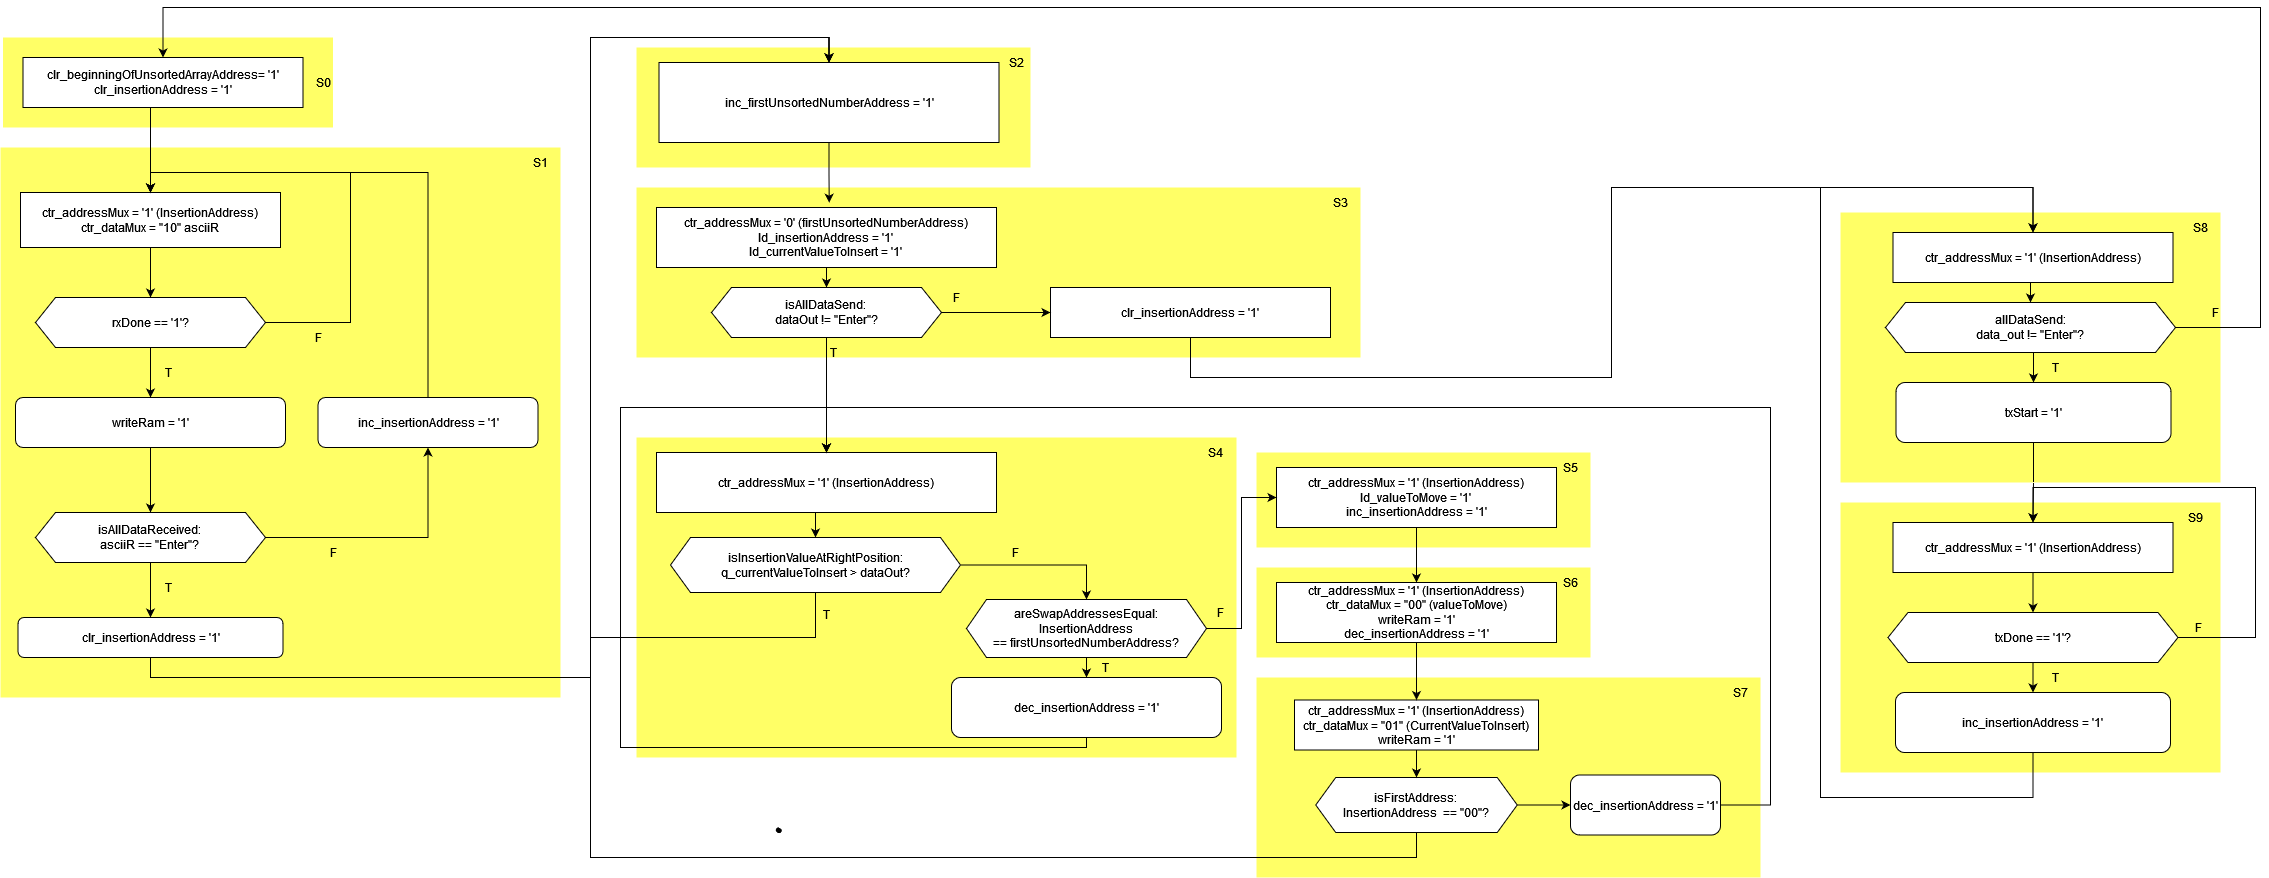
\includegraphics[width=1\linewidth]{Images/ASMDInsertionSort.png}
    \caption{ASMD diagram for the insertion sort}
    \label{fig:asmd}
\end{figure}
\subsection{C coding in Vitis}
Next up, we definied the C program. In order to do so we used the FIR filter project as baseline for Vitis and Vivado and for the code we used a template from the internet \cite{g4g}. We then adapted the template so that we could use the putty.exe as input and output of our unsorted and sorted array. This would then result in the same behaviour like the FSMD and ASIP.\\
In the end we ran our solution on the Zybo Z7 board and could observe the expected behaviour.

\subsection{Create custom IP block}
Lastly, we implemented the IP block. We expected this to be very similar to the C porgram. This was true for the actual InsertionSort functionality. Here, we only did minor adaptions.\\ 
But we encountered other problems: The behaviour for memory allocation and sharing between the host and the FPGA was not how we expected it to be. Additionally, the testbench simulation was not provide the same results as the real tests. Some of our implementations worked within the testbench but not with the real implementation. Lastly, debugging of the file was very difficult. Vitis didn't provide a good debugger. The waveform file was difficult to interpret and print statements could not allways be displayed on the terminal. \\
Due to these findings we had to try a lot of different approaches. We tried to use CharGPT and other large language models. The solution they proposed did not work. In the end we managed to come up with a design on our own that worked just how we expected.

\section{Comparison}
\subsection{Design and Implementation Complexity}
\subsection{Scalability, Flexibility and Reusability}
\subsection{Cost (Development and Production)}
\subsection{Debugging and Verification Complexity}

\section*{Acknowledgment}

The preferred spelling of the word ``acknowledgment'' in America is without 
an ``e'' after the ``g''. Avoid the stilted expression ``one of us (R. B. 
G.) thanks $\ldots$''. Instead, try ``R. B. G. thanks$\ldots$''. Put sponsor 
acknowledgments in the unnumbered footnote on the first page.

\section*{References}
% #TODO why are there two REFERENCES section titles in out pdf?

\printbibliography

\end{document}
